\subsection{Grafische Analyse}\label{subsec:graphical-analysis}

Im Folgenden soll der grundlegende Aufbau der in einem kartesischen Diagramm
entstehenden Formation der Mandelbrot-Menge erörtert als auch eine
Erklärung zur Farbbedeutung gegeben werden.
Zusätzlich zeigt dieses Unterkapitel mit einer exemplarischen Kartografierung
verschiedene, sich wiederholende Bereiche der visuellen Darstellung auf.

\begin{figure}[h!]
  \centering
  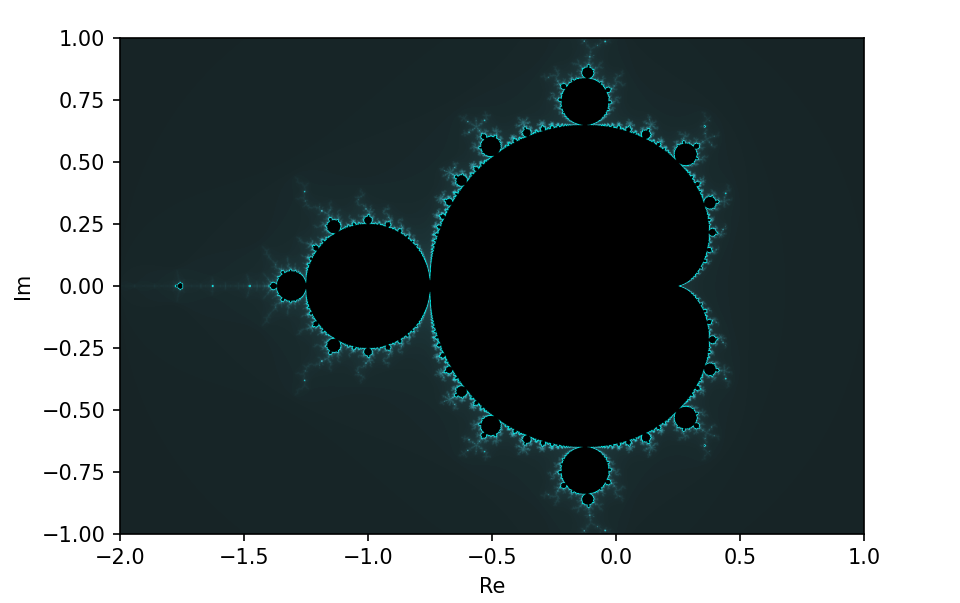
\includegraphics[width=\textwidth]{images/mandelbrotImage}
  \caption[Caption for LOF]{
    Exemplarische Darstellung der Mandelbrot-Menge\footnotemark
  }
  \label{fig:mandelbrot-set}
\end{figure}
% TODO: Add hyperref to code in appendix
\footnotetext{Generiert durch den Code $\cdots$}

Die hier zu sehende Grafik entspricht der Darstellung der Mandelbrot-Menge
in einer komplexen Zahlenebene und wird aufgrund seiner Form
\glqq Apfelm\"annchen\grqq~genannt.
Die zu sehenden, schwarz gefärbten Pixel repräsentieren einen
jeweiligen Wert für $c$, der sich in der Mandelbrot-Menge befindet.
Auffällig ist bei erster Betrachtung, dass sich neben der großen,
einheitlichen Struktur in der Mitte,
deutlich kleinere, ähnlich aussende Formationen um den eigentlichen Hauptkörper
dem Apfelm\"anchen, zum Beispiel im negativen Teil der reellen Achse,
erkennen lassen.
Diese werden \textbf{Satelliten} genannt und existieren aufgrund der Selbstähnlichkeit
der Mandelbrot-Menge in unendlicher Stückzahl - und zwar nicht nur für den Hauptkörper,
sondern auch für jeden Satelliten selbst~\cite{lomonaco_quasi-conformal_2018}.

\subsubsection{Farbbedeutung}

Im Gegensatz zu den ersten grafischen Darstellungen der Mandelbrot-Menge,
auf denen, aufgrund ihrer deutlich geringeren Auflösung,
kleine Satelliten als Druckfehler gewertet wurden\footnote{
  Dies ist eine recht amüsante Anekdote: Während den frühsten Forschungen,
  die Benoît Mandelbrot in den 1970er bei IBM anstellte, war das Drucken deutlich
  mühseliger und aufwendiger, als es heutzutage ist.
  Deshalb existierte ein ganzes Abteil nur für die Herstellung und Bearbeitung von
  Drucks, die - da es damals häufig vorkam - kleine Satelliten am Rande der ersten
  Darstellungen \hyperref[app:5]{[A.5]} gutgemeint wegretuschierten.
  Die ersten Bilder, die Herr Mandelbrot also erhielt, verwunderten ihn sehr und
  er war äußerst aufgebracht, als er von der tolpatschigen Wahrheit erfur
  \cite{numberphile_whats_2019}.
}
und die mit ihrem schwarz-weißen Druck nur zwischen Werte für $c$ \textbf{in}
und \textbf{außerhalb} der Mandelbrot-Menge unterschieden,
besitzt die oben dargestellte
\hyperref[fig:mandelbrot-set]{Figur (\ref{fig:mandelbrot-set})}
einen Farbverlauf.
Dieser, in diesem Fall türkisblaue, Farbgradient gibt an,
wie viele Iterationen es benötigte,
um festzustellen, ob das jeweilige $c$ außerhalb der Mandelbrot-Menge liegt.
Dabei gilt, dass je heller der Pixel beziehungsweise $c$ ist, desto mehr
Iterationen hat es benötigt, um $c$ aus $\mathbb{M}$ auszuschließen\footnote{
  Vgl. z.B. dick markierten Werte für $c_1 = 1 \text{ und } c_3 = 0.5$ in
  \hyperref[tab:iterations-example]{Tabelle~\ref{tab:iterations-example}}.
  $c_1$ ließ sich nach der 3. Iteration aus der Mandelbrot-Menge ausschließen,
  hingegen war dies bei $c_3$ erst nach der 5. Iteration der Fall.
}.
Deshalb existiert ein hell erscheinender Rand um die schwarzen Formationen,
da es für diese Werte außerhalb von $\mathbb{M}$, die sehr nah an tatsächlichen
Werten für $\mathbb{M}$ sind, es viele Iterationen benötigt, um diese auszuschließen.

Neben dieser einen, verhältnismäßig simplen und dementsprechend auf den ersten
Blick aussagekräftigeren Farbkodierung, existiert eine Vielzahl teils deutlich
umfangreicheren Algorithmen, mit denen sich jedoch eine auf das menschliche Auge
ansprechendere Farbgestaltung erzielen lässt.
Diese werden in Kapitel $\cdots$ % TODO: Add \ref to chatper
genauer beschrieben.
Eine Reihe an solchen komplexere Farbverläufe benutzenden Beispielen,
auf die im nächsten Unterkapitel Bezug genommen wird,
lässt sich in \hyperref[app:6]{A.6} betrachten.

\subsubsection{Exemplarische Kartografierung}

Die hingegen von der Farbe unabhängigen, entstehenden Formationen der
Mandelbrot-Menge, die teilweise erst bei sehr kleinen Ausschnitten erkennbar sind,
sind kartografiert und teilweise, wegen einer gewissen Ähnlichkeit, nach
Objekten aus der realen Welt benannt.
So bezeichnet man die größte kreisförmige Kardioide oder auch \glqq Knospe\grqq
~als \glqq K\"orper\grqq~(wobei dieser genauer unterteilt werden kann)
und die daran angrenzende Kardioide als
\glqq Kopf\grqq\footnote{Vgl. \hyperref[app:7]{A.7}}.

Obwohl man jeden Punkt beziehungsweise jeden Ausschnitt einzeln beliebig detailliert
analysieren kann, werden aufgrund der Selbstähnlichkeit Elemente mit ähnlichem
oder gleichen Aufbau erneut aufkehren und dementsprechend gleich benannt.
Im Folgenden soll beispielhaft ein Ausschnitt des in diesem
Video~\cite{beyer_zoomfahrt_2017} gezeigten
\glqq Tal der Seepferdchen\grqq~analysiert werden:

Die Spalte zwischen Kopf und K\"orper wird \glqq Tal der Seepferdchen\grqq
~genannt\footnote{Vgl. \hyperref[app:6.1]{A.6.1}}
~\cite{robert_p_seahorse_2010}, da bei Vergrößerung dieses Ausschnitts
sich unter anschaulicher Farbkodierung auf der rechten Seite
Seepferdchen-ähnliche Formationen erkennen lassen\footnote{Vgl. \hyperref[app:6.2]{A.6.2}}.
Vergrößert man die Sicht auf das Seepferdchen-Tal stark, so lassen sich,
neben weiteren (teils deformierten) Satelliten\footnote{Vgl. \hyperref[app:6.3]{A.6.3}},
bei genauerer Betrachtung des \glqq Seepferdchenschwanzes\grqq~ein
Misiurewicz-Punkt erkennen\footnote{Vgl. \hyperref[app:6.4]{A.6.4}}.
Dieser Misiurewicz-Punkt zeigt ebenfalls die Selbstähnlichkeit der Mandelbrot-Menge auf,
da dieser Punkt sich neben einer Drehung kaum von der eigentlichen
Mandelbrot-Menge unterscheidet~\cite{lei_similarity_1989}.
Vergrößert man diesen Punkt weiter, so findet man erneut einen im Vergleich
zum Apfelm\"annchen sehr ähnlichen aussehenden
Satelliten\footnote{Vgl. \hyperref[app:6.5]{A.6.5}}.